\section{Tuesday, July 2}

\todaybox{We will discuss how to integrate around simple poles, by using the Cauchy Integral Formula.}

Continuing along our integration roadmap, we're going to discuss integrating around poles next. In particular, we're going to discuss simple poles first. For example, how do we find:
$$\int_{|z| = 1} \frac{e^z}{z}dz$$

Since this function isn't analytic inside the curve, the Cauchy Integral Theorem does not apply. We have no reasonable guess as to a primitive (and indeed, this function does not have a primitive on any domain containing the unit circle!). What if we try using the definition of the integral?

\begin{ex}{}{} Let $\gamma(t) = e^{it}$ for $t\in [0,2\pi]$. Then:

$$\int_{\gamma} \frac{e^z}{z}dz = \int_0^{2\pi} \frac{e^{e^{it}}}{e^{it}}ie^{it}dt = i\int_0^{2\pi} e^{\cos(t)}(\cos(\sin(t)) + i\sin(\sin(t)))dt$$

How exactly are we supposed to evaluate this mess of an integral? It doesn't appear likely that any of the techniques from first year calculus will be of much use here.\end{ex}

So, none of our techniques so far work. We need something new. It turns out there is a general theorem that will let us handle any function with a simple pole.

\begin{thmbo}{Cauchy's Integral Formula}{CIF}\index{Cauchy's Integral Formula}
Suppose $f(z)$ is analytic on a domain $D$ such that $\{z\in\C||z-z_0|\le r\} \subset D$. Let $\gamma$ be the circle of radius $r$ centered at $z_0$, travelled once counterclockwise. Then:
$$\int_{\gamma} \frac{f(z)}{z - z_0}dz = 2\pi i f(z_0)$$
\end{thmbo}

Before we prove this, let's see how it applies to our previous example.

\begin{ex}{}{} Let $f(z) = e^z$. This is entire, so is analytic on $\C$. $\C$ is a domain containing $\{z\in\C||z-z_0|\le 1\}$. Let $|z| = 1$ refer to the unit circle travelled once counterclockwise. Then CIF applies to give:

$$\int_{|z| = 1}\frac{e^z}{z}dz = \int_{|z| = 1} \frac{f(z)}{z-0}dz = 2\pi i f(0) = 2\pi i e^0 = 2\pi i$$
\end{ex}

Notice: the theorem is very easy to apply. No complicated arithmetic involved. However, we do need to check the conditions of the theorem before we apply it. This takes some care.

Let's prove this theorem. The proof contains at least one very useful idea.

\begin{proof}Let $\gamma_s$ be the circle of radius $s$ centered at $z_0$, where $s\in(0,r]$. We may assume, without loss of generality, that each $\gamma_s$ starts at the angle $\theta = 0$ and ends at $\theta = 2\pi$. We define a function $F(s)$ as follows:

$$F(s) = \int_{\gamma_s}\frac{f(z)}{z-z_0}dz$$

So the integral we are interested in is $F(r)$. We shall prove two facts about $F(s)$:

\begin{itemize}
\item $F(s)$ is constant on $(0,r]$.
\item $\lim_{s\rightarrow 0^+} F(s) = 2\pi i f(z_0)$.
\end{itemize}

To prove that $F(s)$ is constant, consider the following picture:

\begin{center}
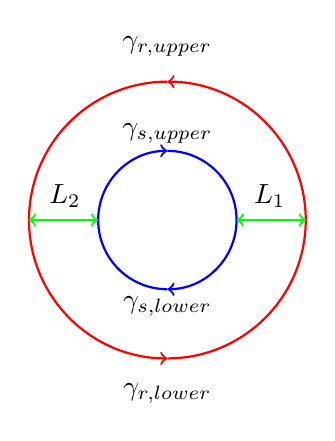
\begin{tikzpicture}

\draw[red, ->, thick] ([shift = (90:50pt)] 0,0) arc (90:270:50pt);
\draw[red, ->, thick] ([shift = (270:50pt)] 0,0) arc (270:450:50pt);
\draw[blue, <-, thick] ([shift = (-90:25pt)] 0,0) arc (-90:90:25pt);
\draw[blue, <-, thick] ([shift = (90:25pt)] 0,0) arc (90:270:25pt);

\draw[green, <->, thick] (0.88,0) -- (1.76,0);
\draw[green, <->, thick] (-0.88,0) -- (-1.76,0);

\draw (0,2.2) node {$\gamma_{r,upper}$};
\draw (0,-2.2) node {$\gamma_{r,lower}$};

\draw (0, 1.1) node {$\gamma_{s,upper}$};
\draw (0, -1.1) node {$\gamma_{s,lower}$};

\draw (1.3,0.3) node {$L_1$};
\draw (-1.3,0.3) node {$L_2$};
\end{tikzpicture}
\end{center}

\noin where $L_1$ and $L_2$ travel from left to right.

Notice that $-\gamma_s = \gamma_{s,upper} + \gamma_{s,lower}$ (since $\gamma_{s,upper}$ and $\gamma_{s,lower}$ are travelling clockwise) and that $\gamma_r = \gamma_{r,upper} + \gamma_{r,lower}$.

Now, we know that $\frac{f(z)}{z-z_0}$ is analytic on $D\setminus \{z_0\}$, which is a domain containing the closed curve $\gamma_{r,upper} + L_2 + \gamma_{s,upper} + L_1$. So by CIT:
$$\int_{\gamma_{r,upper} + L_2 + \gamma_{s,upper} + L_1} \frac{f(z)}{z-z_0}dz = 0$$

And similarly:
$$\int_{\gamma_{r,lower} - L_1 + \gamma_{s,lower} - L_2} \frac{f(z)}{z-z_0}dz = 0$$

Adding these two together gives us that:

\begin{align*}&\int_{\gamma_{r,upper}} \frac{f(z)}{z-z_0} dz + \int_{L_2} \frac{f(z)}{z-z_0} dz + \int_{\gamma_{r,lower}} \frac{f(z)}{z-z_0} dz + \int_{L_1} \frac{f(z)}{z-z_0} dz \\
&+\int_{\gamma_{s,upper}} \frac{f(z)}{z-z_0} dz + \int_{-L_1} \frac{f(z)}{z-z_0} dz + \int_{\gamma_{s,lower}} \frac{f(z)}{z-z_0} dz + \int_{-L_2} \frac{f(z)}{z-z_0} dz  = 0\end{align*}

After simplifying, we find that:

$$\int_{\gamma_{r}} \frac{f(z)}{z-z_0} dz + \int_{-\gamma_{s}} \frac{f(z)}{z-z_0}dz = 0$$

As such, $F(s) = F(r)$ for all $s \in (0,r)$. So $F$ is constant on $(0,r]$.

So, we see that $\lim_{s\rightarrow 0^+} F(s) = \lim_{s\rightarrow 0^+}F(r) = F(r)$.

All that remains is for us to actually compute this limit. To do that, we go to the definition of the integral.

$$\int_{\gamma_s} \frac{f(z)}{z-z_0}dz = \int_0^{2\pi} \frac{f(z_0 + se^{it})}{se^{it}}ise^{it}dt = \int_0^{2\pi} if(z_0 + se^{it})dt$$

We claim that $\lim{s\rightarrow 0^+} \int_0^{2\pi} if(z_0 + se^{it})dt =2\pi i f(z_0)$. Consider the difference:

\begin{align*}\lim{s\rightarrow 0^+} \left|\int_0^{2\pi} if(z_0 + se^{it})dt - 2\pi i f(z_0)\right| &= \lim_{s\rightarrow 0^+} \left|\int_0^{2\pi} if(z_0 + se^{it})dt - \int_0^{2\pi} if(z_0)dt\right|\\
&\le \lim_{s\rightarrow 0^+} \int_0^{2\pi} |f(z_0 + se^{it}) - f(z_0)|dt\\
&\le \lim_{s\rightarrow 0^+} 2\pi \max\{|f(w) - f(z_0)|| w\in \{z\in\C||z-z_0|\le s\}\}
\end{align*}

Now, since $f$ is continuous at $z_0$, we see that  $\lim_{s\rightarrow 0^+}\max\{|f(w) - f(z_0)|| w\in \{z\in\C||z-z_0|\le s\}\} = 0$. So the squeeze theorem gives us that:
$$\lim_{s\rightarrow 0^+} \left|\int_0^{2\pi} if(z_0 + se^{it})dt - 2\pi i f(z_0)\right| = 0$$

As such, $\lim_{s\rightarrow 0^+} \int_0^{2\pi} if(z_0 + se^{it})dt =2\pi i f(z_0)$ as desired.

Putting it all together, we get that:

$$\int_{\gamma_r} \frac{f(z)}{z-z_0}dz = F(r) = \lim_{s\rightarrow 0^+} F(s) = 2\pi i f(z_0)$$

\end{proof}

While technical, this proof has a really important idea. The technique for showing that the integrals over the two circles are equal is fairly useful. For example:

\begin{ex}{}{}Let $\gamma$ be the circle of radius $3$ centered at $0$, travelled once counterclockwise. Find $\int_{\gamma} \frac{1}{z-1}dz$.

As written, CIF doesn't apply. This first version of CIF only applies to circles centered at $z_0$, which in this case is $1$.

However, our technique from the proof of CIF gives that:

$$\int_{\gamma} \frac{1}{z-1}dz = \int_{|z-1|=1} \frac{1}{z-1}dz$$

And now we're in a situation where CIF applies. It gives $\int_{\gamma} \frac{1}{z-1}dz = 2\pi i$.\end{ex}